\section{Evaluation} \label{sec:eval}

%% Recap work flow for readers
To evaluate our compilation flow and network architectures, we use a set of benchmarks implemented in Spatial. 
%We connect the Spatial's output IR with our low-level compiler described in section~\ref{sec:compiler}.
We start with Spatial's output IR (Section~\ref{sec:compiler}), and transform it into a graph of distributed, streaming VBs.
Our compiler then performs place and route for a target architecture before generating a configuration for cycle-accurate simulation. 
During simulation, we track the amount of data moved by each switch and router, which we integrate with synthesis results to produce estimates of area and power.

For each application, we find the highest-performing parallelization and tiling factors; for DRAM-bound applications, this is the configuration that saturates memory bandwidth.
The optimum parameters for each network configuration may vary, as high parallelization does not improve performance on a low bandwidth network.
%Next, for each optimized application, we evaluate network configurations as described in Section~\ref{sec:net_dse}.
We start with benchmark characterizations (Section~\ref{sec:app_char}), analyzing application characteristics and communication patterns to identify how they interact with networks.
Next, we characterize the area and energy of network primitives, which we use to calculate the total network area and energy in Section~\ref{sec:net_char}. 
Finally, Section~\ref{sec:network} presents a design space study over all network dimensions for both pipelined and scheduled architectures. 
Table~\ref{tab:notation} summarizes the notation we use to describe network configurations in the remainder of this section.

\subsection{Application Characterization} \label{sec:app_char}

\begin{figure}
\centering
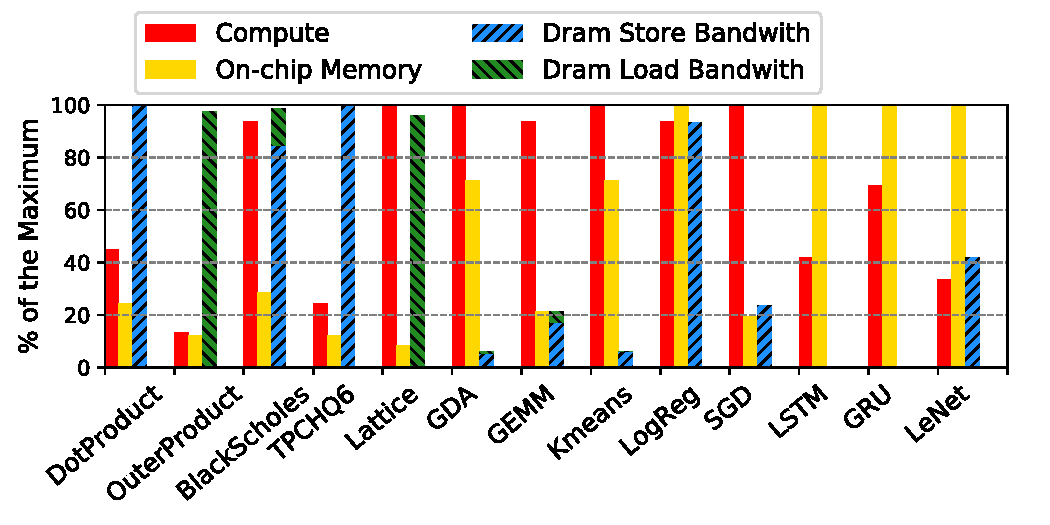
\includegraphics[width=1\columnwidth]{figs/util_bw2.pdf}
\caption{Physical resource and bandwidth utilization for various applications.}\label{fig:util_bw}
\centering
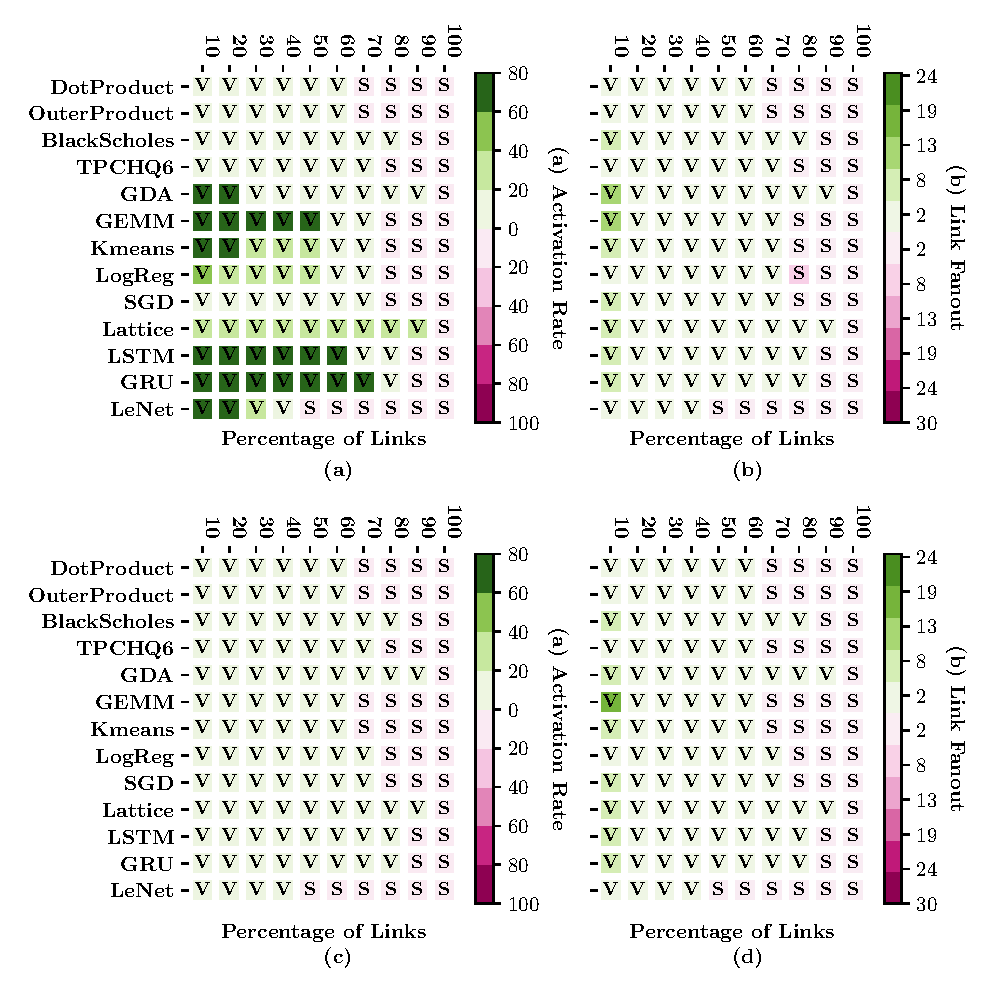
\includegraphics[width=1\columnwidth]{figs/link7.pdf}
  \caption{Application communication patterns on pipelined (a,b) and scheduled (c,d) CGRA architectures.
  (a) and (c) show the activation rate distribution of logical links at runtime. 
  Links sorted by granularity, then rate; darker boxes indicate higher rates.
  The split between green and pink shows the ratio of logical vector to scalar links. (b) and (d) show the distribution of broadcast link fanouts.
 }\label{fig:link}
\end{figure}

\begin{figure}
\centering
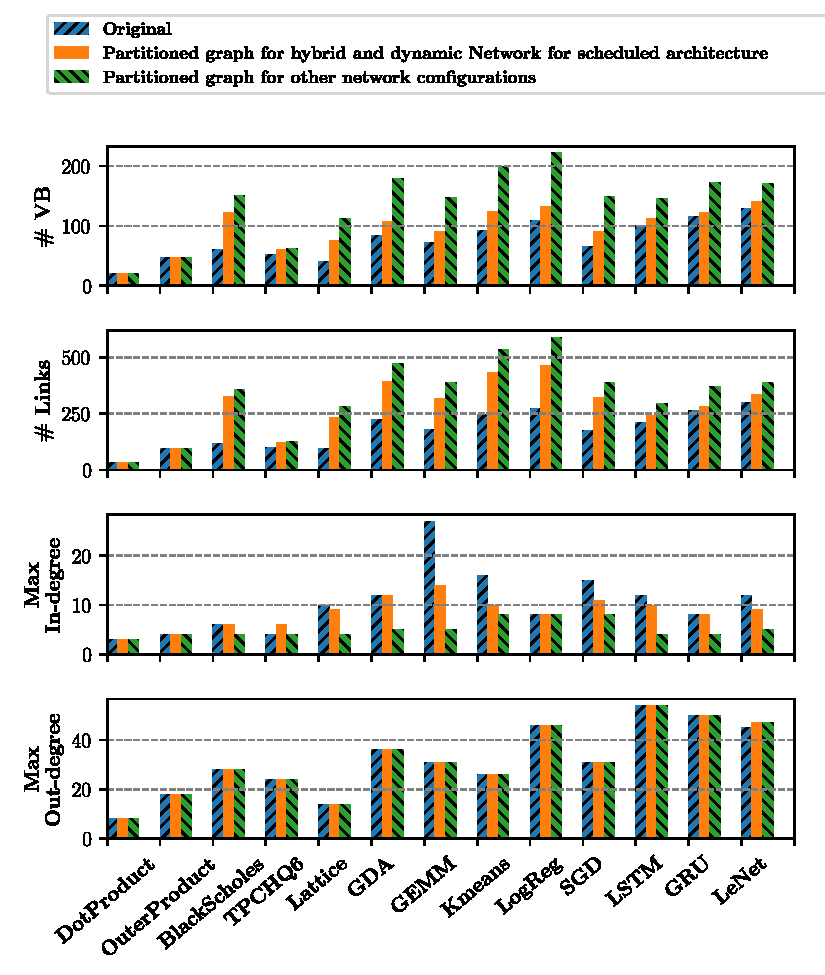
\includegraphics[width=1\columnwidth]{figs/graph.pdf}
\caption{Characteristics of program graphs.}\label{fig:graph}
\end{figure}

We select a mix of applications from domains where hardware accelerators have shown promising performance and energy-efficiency benefits, such as linear algebra, databases, and machine learning.
Table~\ref{tab:benchmark} lists the applications and their data size.
Figure~\ref{fig:util_bw} shows, for each design, which resource limits performance: compute, on-chip memory, or DRAM bandwidth. 
%Variations in these application characteristics introduce different on-chip network requirements.
DotProduct, TPCHQ6, OuterProduct, and BlackScholes are DRAM bandwidth-bound applications. 
These applications use few on-chip resources to achieve maximum performance, resulting in minimal communication.
Lattice (a fast inference model for low-dimensional regression~\cite{garcia2009lattice}), GDA, Kmeans, SGD, and LogReg are compute-intensive applications; for these, maximum performance requires using as much parallelization as possible. 
Finally, LSTM, GRU, and LeNet are applications that are limited by on-chip memory bandwidth or capacity. 
For compute- and memory-intensive applications, high utilization translates to a large interconnection network bandwidth requirement to sustain application throughput. 

Figure~\ref{fig:link}(a,b) shows the communication pattern of applications
characterized on the pipelined CGRA architecture, including the variation in communication granularity. 
Compute and on-chip memory-bound applications show a significant amount of high-bandwidth communication (links with almost 100\% activity). 
A few of these high-bandwidth links also exhibit high broadcast fanout. 
Therefore, a network architecture must provide sufficient bandwidth and efficient broadcasts to sustain program throughput.
On the contrary, time-scheduled architectures, shown in Figure~\ref{fig:link}(c,d), exhibit
lower bandwidth requirements due to the lower throughput of individual compute PBs. 
Even applications limited by on-chip resources have less than a 30\% firing rate on the busiest logical links; this reveals an opportunity for link sharing without sacrificing performance.

Figure~\ref{fig:graph} shows statistics describing the VB dataflow graph before and after partitioning.
The blue bars show the number of VBs, number of logical links, and maximum VB input/output degrees in the original parallelized program; the yellow and green bars show the same statistics after partitioning. 
Fewer VBs are partitioned for hybrid networks and dynamic networks with the time-scheduled architecture, as explained in Section~\ref{sec:partition}. 
The output degree does not change with partitioning because most outputs with a large degree are from broadcast links.

\subsection{Area and Energy Characterization} \label{sec:net_char}

Figure~\ref{fig:sweep} shows that switch and router power scale linearly with the rate of data transmission, but that there is non-zero power at zero-load. 
For simulation, the duty cycle refers to the amount of offered traffic, not accepted traffic.
Because our router uses a crossbar without speedup \cite{dallytowles}, the testbench saturates the router at 60\% duty cycle when providing uniform random traffic. 
Nonetheless, router power still scales linearly with accepted traffic.

A sweep of different switch and router parameters is shown in Figure~\ref{fig:char}. Subplots (d,e,f) show the energy necessary to transmit a single bit through a switch or router.
Subplot (a) shows the roughly quadratic scaling of switch area with the number of links between adjacent switches.
Vector switches scale worse with increasing bandwidth than scalar switches, mostly due to increased crossbar wire load. 
At the same granularity, a router consumes more energy a switch to transmit a single bit of data, even though the overall router consumes less power (as shown in Figure~\ref{fig:sweep}); 
this is because the switch has a higher throughput than the router.
The vector router has lower per-bit energy relative to the scalar router because it can amortize the cost of allocation logic, whereas the vector switch has higher per-bit energy relative to the scalar switch due to increased capacitance in the large crossbar. 
Increasing the number of VCs or buffer depth per VC also significantly increases router area and energy, but reducing the router flit width can significantly reduce router area. 

Overall, these results show that scaling static bandwidth is cheaper than scaling dynamic bandwidth, and a dynamic network with small routers can be used to improve link sharing for low bandwidth communication.  
We also see that a specialized scalar network, built with switches, adds negligible area compared to and is more energy efficient than the vector network. 
Therefore, we use a static scalar network with a bandwidth of 4 for the remainder of our evaluation, except when evaluating the pure dynamic network.
The dynamic network is also optimized for the rare instances when the static scalar network is insufficient. 
When routers transmit scalar data, the high bits of data buffers are clock-gated, reducing energy as shown in (f).
Figure~\ref{fig:area} summarizes the area breakdown of all the network configurations that we evaluate.
\subsection{Network Architecture Exploration} \label{sec:net_dse}

\begin{table}
\footnotesize
\begin{tabular*}{\columnwidth}{p{1cm} p{7cm}}
  \bottomrule
  \textbf{Notation} & \textbf{Description} \\\midrule
  $[$S,H,D$]$ & Static, hybrid, and dynamic network \\\midrule
  x\# & Static bandwidth on vector network (\#links between switches) \\\midrule
  %$s\#$ & Number of links between switches on static scalar network \\\midrule
  f\# & Flit width of a router or vector width of a switch \\\midrule
  v\# & Number of VC in router \\\midrule
  b\# & Number of buffers per VC in router \\\midrule
  $[$db,cd$]$ & Buffered vs. credit-based flow control in switch \\\midrule
  %$[Scheduled, Pipelined]$ & Time scheduled vs deep pipelined accelerator architectures \\\midrule
\end{tabular*}
\caption{Network design parameter summary.}
\label{tab:notation}
\end{table}
\begin{figure}
\centering
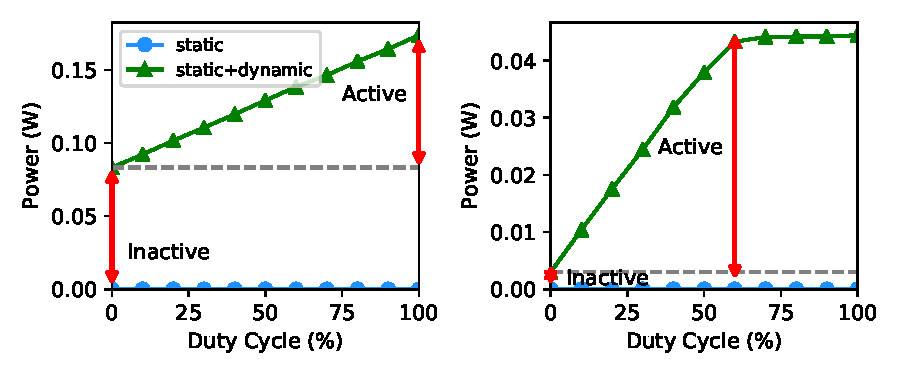
\includegraphics[width=1\columnwidth]{figs/sweep.pdf}
  \caption{Switch and router power with varying duty cycle.}\label{fig:sweep}
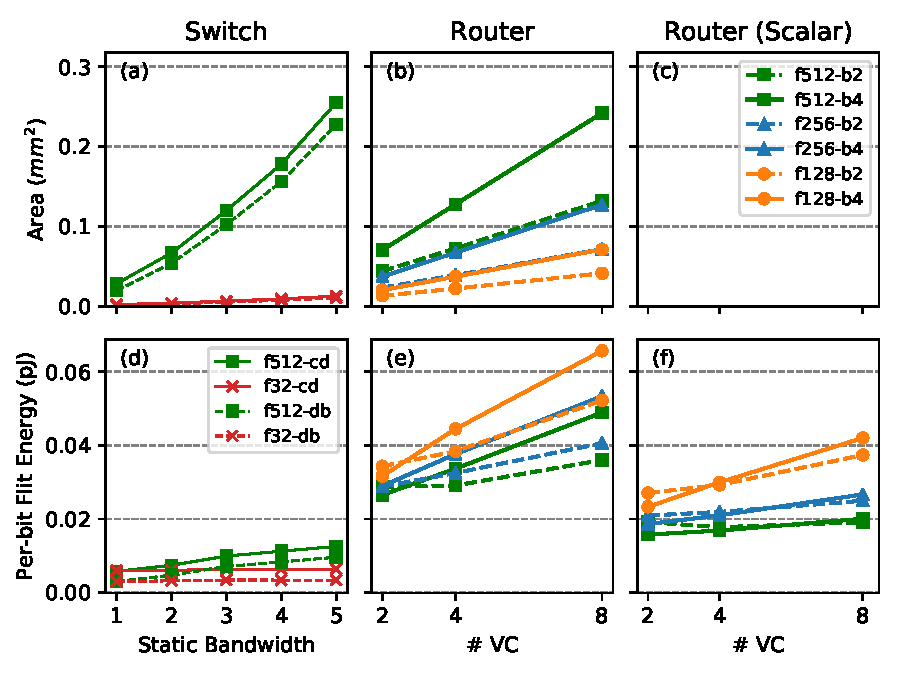
\includegraphics[width=1\columnwidth]{figs/char.pdf}
  \caption{Area and per-bit energy for (a,d) switches and (b,c,e,f) routers. 
  (c,f) Subplots (c,f) show area and energy of the vector router when used for scalar values (32-bit).}\label{fig:char}
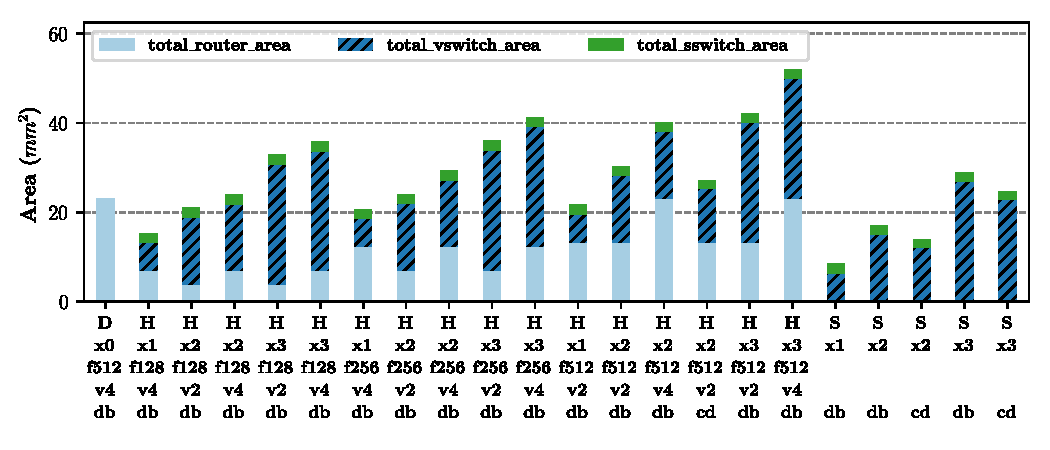
\includegraphics[width=1\columnwidth]{figs/area.pdf}
  \caption{Area breakdown for all network configurations.}\label{fig:area}
\end{figure}

We evaluate our network configurations in five dimensions: performance (perf), performance per network area (perf/area), performance per network
power (perf/watt), network area efficiency (1/area), and network power efficiency (1/power). 
Among these metrics, performance is the most important: networks only consume a small fraction of the overall accelerator area and energy (roughly 10-20\%). 
Because the two key advantages of hardware accelerators are high throughput and low latency, 
we filter out a network design point if it introduces
more than 10\% performance overhead.
This is calculated by comparing to an ideal network with infinite bandwidth and zero latency.

For metrics that are calculated per application, such as performance, performance/watt, and power efficiency, we first normalize the metric with respect to the 
worst network configuration for that application. 
For each network configuration, we present a geometric mean normalized across all applications. 
For all of our experiments, except Section~\ref{sec:scale}, we use a network
size of $14\times14$ end-point PBs. All vector networks use a vectorization factor of 16 (\SI{512}{bit} messages).

\begin{figure}
\centering
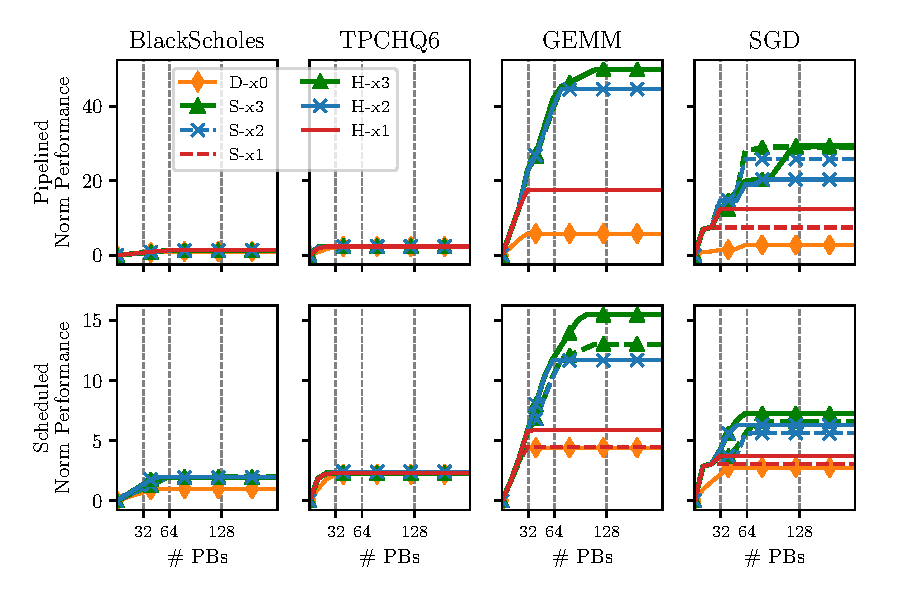
\includegraphics[width=1\columnwidth]{figs/scale.pdf}
\caption{Performance scaling with increased CGRA grid size for different networks.}\label{fig:scale}
\end{figure}
\subsubsection{Bandwidth scaling with network size}\label{sec:scale}
%Figure~\ref{fig:scale} shows the performance scaling of applications as accelerator size scales with different network configurations.
Figure~\ref{fig:scale} shows how different networks allow several applications to scale to different numbers of PBs.
For IO-bound applications (BlackScholes and TPCHQ6), performance does not scale with additional compute and on-chip memory resources.
However, the performance of compute-bound applications (GEMM and SGD) improves with increased resources, but plateaus at a level that is determined by on-chip network bandwidth. 
%Although this is expected for general network designs, it is much more noticeable due to the high-bandwidth communication inherent in pipelined reconfigurable accelerators.
This creates a trade-off in accelerator design between highly vectorized compute PBs with a small network---which would be underutilized for non-vectorized problems---and smaller compute PBs with limited performance due to network overhead. 
For more finely grained compute PBs, both more switches and more costly (higher-radix) switches must be employed to meet application requirements.

The scaling of time-scheduled accelerators (bottom row) is much less dramatic than that of deeply pipelined architectures (top row). 
Although communication between PBs in these architectures is less frequent, the scheduled architecture must use additional parallelization to match the throughput of the pipelined architecture; this translates to larger network sizes. 
%Since scaling dynamic bandwidth is much more expensive than scaling static bandwidth, as shown in section \ref{sec:net_char}, 
%we only explored scaling bandwidth in vector switches. 

For pipelined architectures, both hybrid and static networks provide similar scaling with the same static bandwidth:
the additional bandwidth from the dynamic network in hybrid networks does not provide additional scaling. 
This is mostly due to a bandwidth bottleneck between a PB and its router, which prevents the PB from requesting multiple elements per cycle.
Hybrid networks tend to provide better scaling for time-scheduled architectures; multiple streams can be time multiplexed at each ejection port without losing performance.

\begin{figure}
\centering
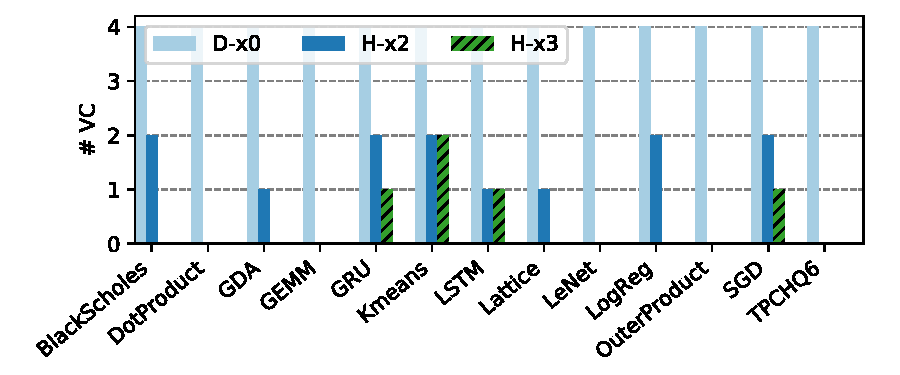
\includegraphics[width=1\columnwidth]{figs/vc.pdf}
  \caption{Number of VCs required for dynamic and hybrid networks. (No VCs indicates that all traffic is mapped to the static network.)}\label{fig:vc}
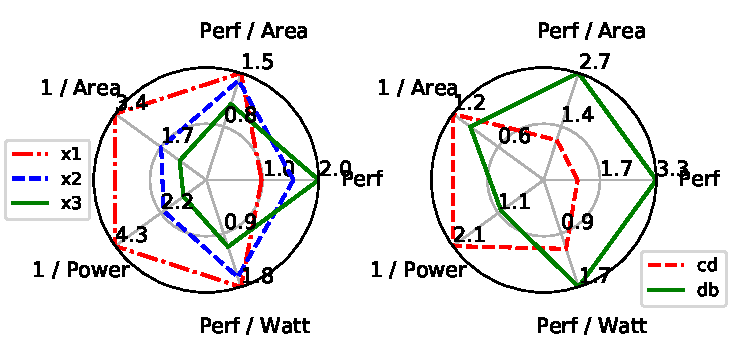
\includegraphics[width=1\columnwidth]{figs/radar_switch.pdf}
  \caption{
    Impact of bandwidth and flow control strategies in switches.}\label{fig:radar_switch}
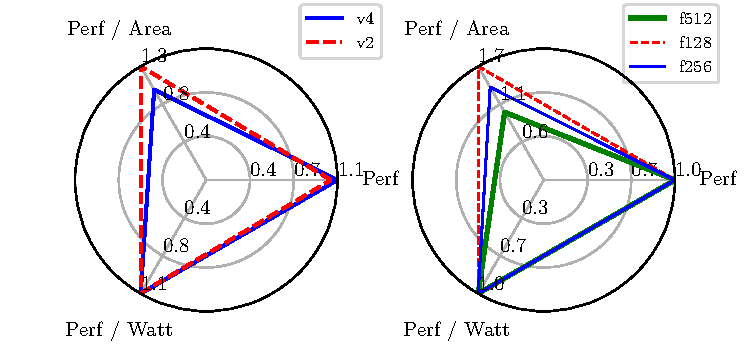
\includegraphics[width=1\columnwidth]{figs/radar_router.pdf}
  \caption{Impact of VC count and flit widths in routers.}\label{fig:radar_router}
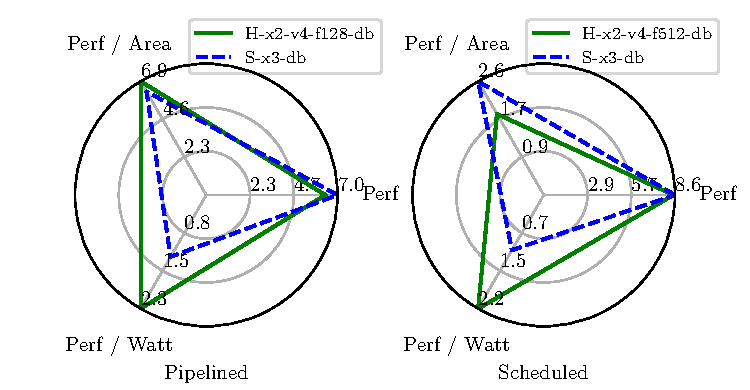
\includegraphics[width=1\columnwidth]{figs/radar_best.pdf}
  \caption{Geometric mean improvement for the best network configurations, relative to the worst configuration.}\label{fig:radar_best}
\end{figure}

\begin{figure*}
\centering
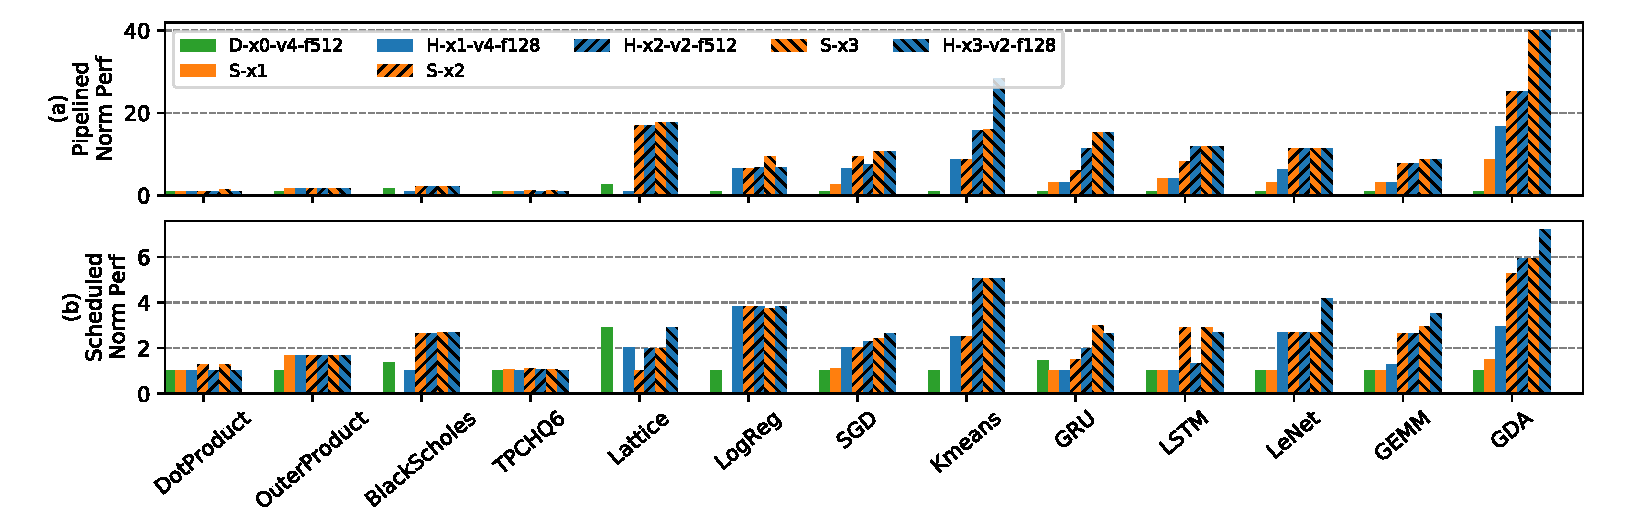
\includegraphics[width=1\linewidth]{figs/perf.pdf}
  \caption{Normalized performance for different network configurations.}\label{fig:perf}
\end{figure*}

\begin{figure}
\centering
  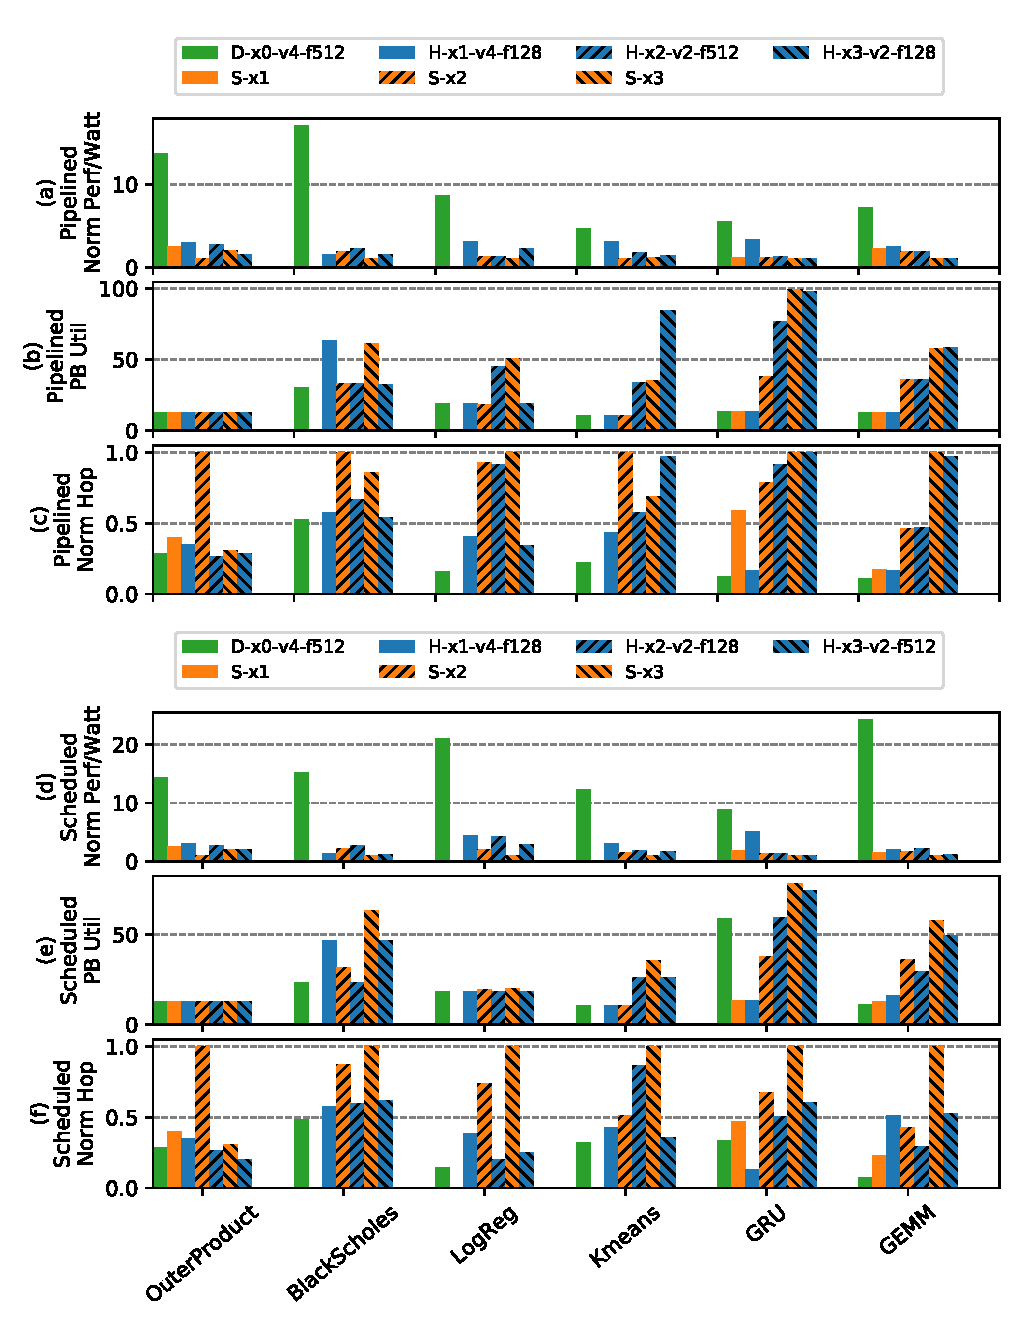
\includegraphics[width=1\columnwidth]{figs/energy.pdf} 
\caption{(a,d): Normalized performance/watt. (b,e): Percentage of compute and memory PBs utilized for each network configuration. 
  (c,f): Total data movement (hop count).}
\label{fig:energy}
\end{figure}

\subsubsection{Bandwidth and flow control in switches}

In this section, we study the impact of static network bandwidth and flow control mechanism (per-hop vs. end-to-end credit-based). 
On the left side of Figure~\ref{fig:radar_switch}, we show that increased static bandwidth results in a linear performance increase and a superlinear increase in area and power. 
As shown in Section~\ref{sec:scale}, any increase in accelerator size must be coupled with increased network bandwidth to effectively scale performance. 
This indicates that network overhead will increase with the size of an accelerator.

The right side of Figure~\ref{fig:radar_switch} shows that, although credit-based flow control reduces the amount of buffering in switches and decreases network area and energy, application performance is significantly impacted. 
This is the result of imbalanced data-flow pipelines in the program: when there are parallel long and short paths over the network, there must be sufficient buffer space on the short path equal to the product of throughput and the difference in latency. 
Because performance is our most important metric, credit-based flow control is not feasible, especially because the impact of bubbles increases with communication distance, and therefore network size.

\subsubsection{VC count and reduced flit width in routers}
In this experiment, we study the area-energy-performance trade-off between routers with different VC counts. As shown
in Section~\ref{sec:net_char}, using many VCs increases both network area and energy.
However, using too few VCs may force roundabout routing on the dynamic network or result in VC allocation failure when the network is heavily utilized.
Nonetheless, the left side of Figure~\ref{fig:radar_router} shows minimal performance improvement from using more VCs. 

Therefore, for each network design, we use a VC count equal to the maximum number of VCs required to map all applications to that network. 
Figure~\ref{fig:vc} shows that the best hybrid network configurations with 2x and 3x static bandwidth require at most 2 VCs, whereas the pure dynamic network requires 4 VCs to map all applications.
%This is different from a traditional processor based (request-response) architecture because, first, less VCs are required to map a large amount of traffic onto dynamic network due deadlock challenges
%specific to streaming architectures, second, communication is much infrequent to incur bandwidth penalty on dynamic network. 
Because dynamic network communication is infrequent, hybrid networks with fewer VCs provide both better energy and area efficiency than networks with more VCs, even though this constrains routing on the dynamic network.
%The improvement is less significant in a time-scheduled architecture because of an overall reduction in required bandwidth.

We also explore the effects of reducing dynamic network bandwidth by using smaller routers;
as shown in Section~\ref{sec:net_char}, routers with smaller flits have a much smaller area.
Ideally, we could scale static network bandwidth while using a low-bandwidth router to provide an escape path and reduce overall area and energy overhead. 
The right side of Figure~\ref{fig:radar_router} shows that, for a hybrid network, reducing flit width improves area efficiency with minimal performance loss. 

%The reduction in performance is more significant in pipelined CGRAs than time-scheduled CGRAs, as the latter has a lower bandwidth requirement.

\subsubsection{Static vs. hybrid vs. dynamic networks}

Figure~\ref{fig:perf} shows the normalized performance for each application running on several network configurations.
%For some applications, the ideal configuration could not be placed and routed onto a static network with 1x bandwidth; missing bars for S-x1 are the result of these failures.
For some applications, the bar for S-x1 is missing; this indicates that place and route failed for all unrolling factors.
For DRAM-bound applications, the performance variation between different networks is trivial because only a small fraction of the network is being used. 
In a few cases (Kmeans and GDA), hybrid networks  provide better performance due to slightly increased bandwidth.
For compute-bound applications, performance primarily correlates with network bandwidth because more bandwidth permits a higher parallelization factor. 

%Figures~\ref{fig:energy} [1,4] show the normalized performance/watt of the network for pipelined and scheduled
%architectures. Figure [2,5] show the corresponding PB utilizations in the network. Figure [3,6] summarize the total
%data movement distributed on static vector, static scalar, dynamic vector and dynamic scalar for that network
%configuration.  
The highest bandwidth static network uses the most PBs, as shown in Figures~\ref{fig:energy}(b,e), because it permits more parallelization. 
It also has more data movement, as shown in (c,f), because PBs can be distributed farther apart. 
Due to bandwidth limitations, low-bandwidth networks perform best with small unrolling factors---they are unable to support the bisection bandwidth of larger program graphs.
This is evident in Figures~\ref{fig:energy}(b,e), where networks D-x0-v4-f512 and S-x2 have small PB utilizations.

With the same static bandwidth, most hybrid networks have better energy efficiency than the corresponding pure static networks, even though routers take more energy than switches to transmit the same amount of data.
This is a result of allowing a small amount of traffic to escape onto the dynamic network: with the dynamic network as a safety net, static place and route tends to converge to better placements with less overall communication.
This can be seen in Figures~\ref{fig:energy}(c,f), where most static networks have larger hop counts than the corresponding hybrid network; hop count is the sum of all runtime link traversals, normalized per-application to the network configuration with the most hops.
Subplots (e,f) show that more PBs are utilized with static networks than hybrid networks.
%Compared to hybrid networks, (e,f), show larger PB utilization at the same parallelization factor on the purely static network .
This is because the compiler imposes less stringent IO constraints on PBs when partitioning for the hybrid network (as explained in Section~\ref{sec:partition}), which results in fewer PBs, less data movement, and greater energy efficiency for hybrid networks.

In Figure~\ref{fig:radar_best}, we summarize the best perf/watt and perf/area (among network configurations with <10\% performance overhead) for pipelined and scheduled CGRA architectures. 
Pure dynamic networks are not shown because they perform poorly due to insufficient bandwidth.
On the pipelined CGRA, the best hybrid network provides a 6.4x performance increase, 2.3x better energy efficiency, and a 6.9x perf/area increase over the worst network configuration. 
The best static network provides 7x better performance, 1.2x better energy efficiency, and 6.3x better perf/area. 
The hybrid network gives the best perf/area and perf/watt, with a small degradation in performance when compared to the static network. 
On the time-scheduled CGRA, both static and hybrid networks have an 8.6x performance improvement. 
The hybrid network gives a higher perf/watt improvement at 2.2x, whereas the static network gives a higher perf/area improvement at 2.6x.
Overall, the hybrid networks deliver better energy efficiency with shorter routing distances by allowing an escape path on the dynamic network.

%It can also provide a decent area efficiency when coupled with a small dynamic network with a minimum performance penalty. 

%\begin{figure}[ht]
%\centering
%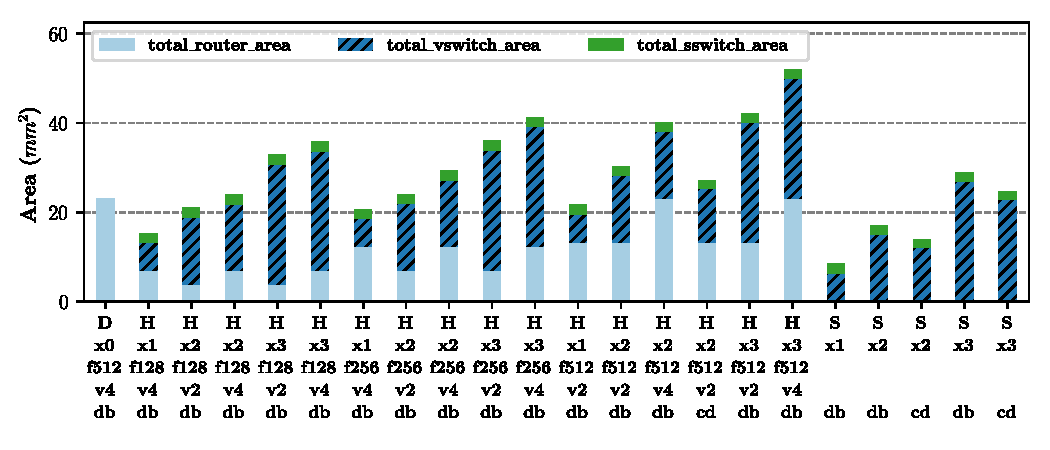
\includegraphics[width=\columnwidth]{figs/area.pdf}
%\caption{Area breakdown of network architectures}\label{fig:area}
%\end{figure}

%In this section, we evaluate the proposed network architecture design points from Section~\ref{sec:network}, summarized in Table~\ref{tab:net_dse}.
%Pure dynamic networks are represented with $D{\dash}v0{\dash}s0$, indicating no static links in the network. 
%Pure static networks are prefixed with $v\#{\dash}s\#$, where the $\#$ are number of
%scalar and vector links between switches. Hybrid networks are shown as $D{\dash}v\#{\dash}s\#$.
%Figure~\ref{fig:area_vc} (a) shows the number of VCs required to map each application for architectures containing a dynamic network. 
%%The maximum number of VCs required across all applications is the number of VCs we use to account for area. 
%When computing area for each configuration, we use the maximum number of VCs required to map any application.
%For application in hybrid network with no VCs, all traffic is mapped onto the static network.

%Figure~\ref{fig:area_vc} (b) shows the area breakdown of the architecture. 
%For $D{\dash}v0{\dash}s0$, all links are routed through the dynamic network, resulting in heavy congestion and a large VC requirement. 
%Consequently, the large number of VCs directly contribute to the large router area. 
%All the other dynamic configurations only need 2 VCs to avoid deadlock. 
%The network area contributes only a small fraction of the overall area, but using a dynamic network with a smaller flit width saves router area roughly linearly.
%%The hybrid network $D{\dash}v1{\dash}s4-f512, and D{\dash}v2{\dash}s4-f512$ has slightly larger area than their equivalent bandwidth counterpart design point in static network $v2{\dash}s4$ and $v3{\dash}s4$ due to the overhead on dynamic routing and buffering. 

%Figure~\ref{fig:slow_down} (a) shows the performance degradation normalized to the ideal network with infinite buffers; all the other design points have an end-point buffer with depth 4 inside the CUs.
%We found that for memory bandwidth bound applications, the performance is roughly the same across all design points, mostly due to the low CU utilization and lack of congestion. 
%Although BlackScholes is DRAM bandwidth bound, the inner loop partition introduces lots of CUs communicating their temporary results. 
%The slow-down with BlackScholes with static network compared to ideal network is due to the pipeline bubbles introduced by VB partitioning as explained in Section \ref{sec:network}. 

%Overall, the hybrid network with the $v1$ static network has a slowdown of less than 2x overall, while the hybrid network with $v2$ has static-equivalent performance.

%The static network with credit-based flow control suffers from insufficient end-point buffers for most applications, resulting in poor performance. 
%The slowdown in dynamic and hybrid networks is mostly due to the high-throughput broadcasts and congestion. 
%Figure~\ref{fig:slow_down} (b) shows the slowdown normalized to total area. 
%Since the network only takes a small fraction of the chip area, the trends is similar to performance. 

%Figure~\ref{fig:slow_down}(c) shows the network energy normalized to $v2{\dash}s4$. 
%The pure dynamic network consumes the most energy because of the amount of buffers and the router's inherently higher per-flit energy. 
%Breaking down the hybrid network energy, we can see that vast majority of communication is mapped to the static network. 
%There is a small gap between energy on $v2{\dash}s4$ and $D{\dash}v2{\dash}s4$, where the hybrid consumes less energy, even though all traffic is mapped onto the static network. 
%Another outlier on LeNet $D{\dash}v2{\dash}s4$ consumes more energy then $v2{\dash}s4{\dash}db$ is likely introduced by randomness from the iterative placer. 
%These are discrepancies introduced by different placements having different distances between nodes.
%It is also important to note hat the overprovisioned static capacity has a high (31\%) mean energy cost, even though it is not being used.
%%This is due to a limitation in current implementation that pure static networks are placed and routed with only back tracking placer, while the hybrid is also using the iterative placer. 
%%As a result, we found better mapping on hybrid network which reduce the hop distance on links, which is not essential for slowdown but directly translates into energy. 
%%However, in theory we should be able to use both algorithm on all design points. 

%In Figure~\ref{fig:slow_down} (d), we show the normalized power. 
%Here, design points with large slowdown naturally have lower power, such as $v3{\dash}s4{\dash}cd$. 
%However, we also show that the network is consuming only a very small portion of the power compared with the compute tiles. 
%The network only consumes around 0--3 W of energy compared to the theoretical peak Plasticine power of 49W.
%Therefore, among the metrics of performance, area, and power, performance is the most important metric to measure the network architectures. 

%%
%%This allows it to be stored in the smaller buffers without any translation logic, and does not result in a loss of throughput (the throughput would be limited regardless at the non-priority VC).
%%Because the priority VC is considered in route scoring, the placer is able to ensure that less than 1\% of traffic in the worst app (XXX) traverses non-priority VCs.
%%This scheme results in a XXX\% lower network area, with a geometric mean slowdown of XXX\% (worst XXX\%).
